\documentclass[a4paper,12pt]{article}

\usepackage{amssymb}
\usepackage{amsmath}
\usepackage{amsfonts}
\usepackage{txfonts}
\usepackage{upgreek}
\usepackage{graphicx}
\usepackage{siunitx}
\usepackage{enumerate}
\usepackage[left=2cm,right=2cm,top=2cm,bottom=2cm]{geometry}

\usepackage[obeyspaces]{url}

%\newcommand{\question}[2]{\textbf{\textit{#1}}\quad{\footnotesize\textit{(#2 points)}}\\[3mm]}
\newcommand{\question}[1]{\textbf{\textit{#1}}}
\newcommand{\points}[1]{\quad{\footnotesize\textit{(#1 points)}}}
\newcommand{\point}{\quad{\footnotesize\textit{(1 point)}}}
\newcommand{\HRule}{\rule{\linewidth}{0.3mm}}
\newcommand{\dd}{\mathrm{d}}
\renewcommand{\pi}{\uppi}
\newcommand{\ii}{\mathrm{i}}
\renewcommand{\thefootnote}{\normalsize\fnsymbol{footnote}}
\DeclareMathOperator{\e}{e}
\newcommand{\bra}{\langle}
\newcommand{\ket}{\rangle}

\renewcommand{\theequation}{\Roman{equation}}

\begin{document}
\pagestyle{empty}

\begin{center}
\LARGE \textbf{Astronomy from 4 perspectives: the Dark Universe}
\HRule
\end{center}
\begin{flushright}
prepared by: Florence participants and BMS
\end{flushright}
\begin{center}
{\Large \textbf{play with data: Supernova-cosmology and dark energy}}
\end{center}
\vspace{5mm}

\noindent
The Supernova Cosmology Project observed supernovae of the type Ia in distant galaxies, determined the distance modulus by measuring the apparent brightness as well as the redshift of the host galaxy. From the relation between distance and redshift one can measure the density parameters $\Omega_X$ and the dark energy equation of state $w$. The exercise sheet uses data from A. Goobar et al., PhST, 85, 47 (2000).

\begin{enumerate}[\itshape \bfseries 1.]

\item \question{distance redshift-relationships in FLRW-universes}\\
In this exercise you can play with SCP-data and explore the sensitivity of the supernova brightness on the cosmological parameters. Please have a look at the python-script \path{supernova_plot.py}, which reads the data file from SCP and plots distance modulus $\mu$ as a function of redshift $z$. The cosmological model is a spatially flat FLRW-cosmology with the Hubble function
\begin{equation}
H(z) = H_0\sqrt{\Omega_m(1+z) + (1-\Omega_m)(1+z)^{3(1+w)}}
\end{equation}
where the density of the dark energy component is automatically set to $\Omega_X=1-\Omega_m$ to enforce flatness. Setting $w=-1$ recovers the case of the cosmological constant $\Lambda$, in which case $\Omega_X=\Omega_\Lambda$.

\begin{enumerate}[(a)]
\item{Start by guessing different values for $\Omega_m$ to find the best value: What's $\Omega_\Lambda$?}
\item{What's your explanation why $\Lambda$ makes the supernovae dimmer?}
\end{enumerate}

\begin{figure}[h]
\begin{center}
\resizebox{9cm}{!}{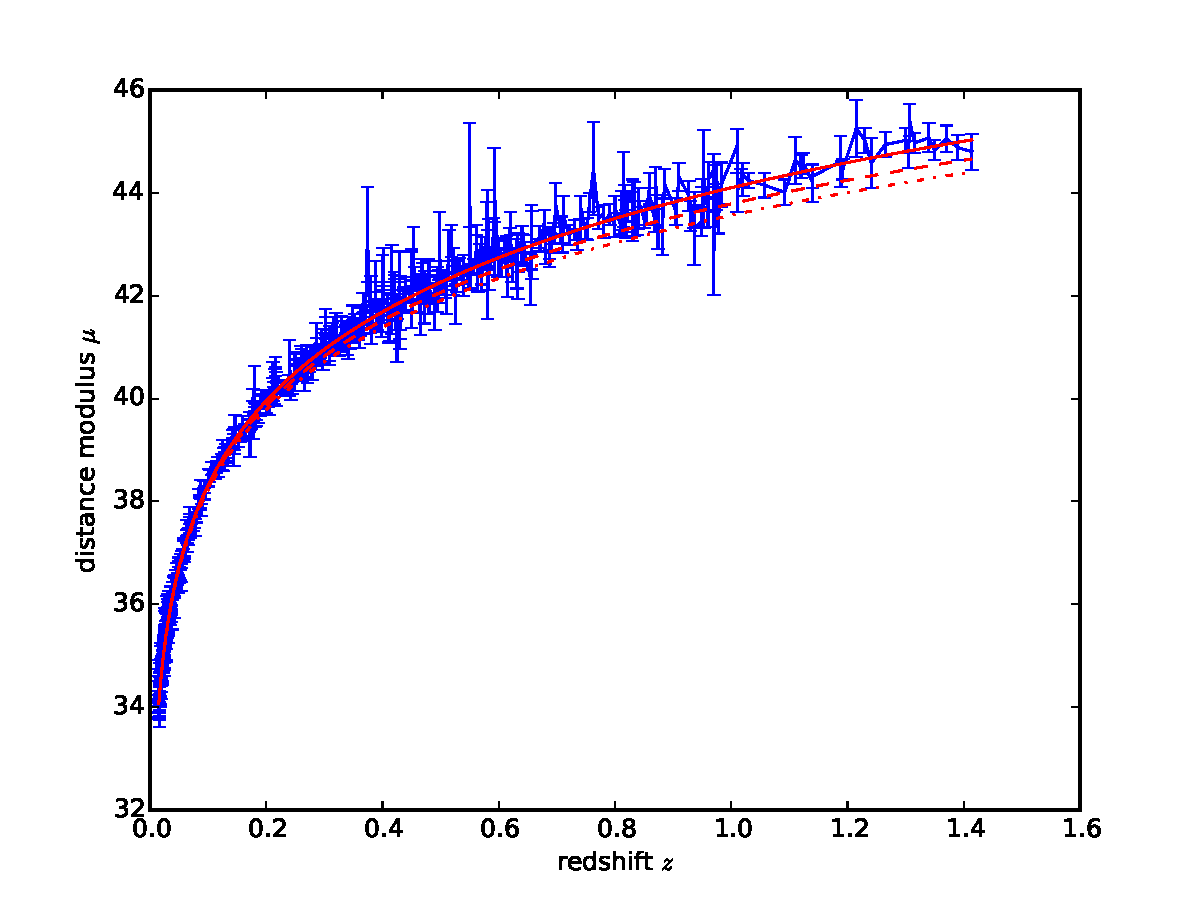
\includegraphics{./figures/supernova_plot.pdf}}
\caption{data from the SCP and distance redshift relationships with varying $\Omega_m$}
\end{center}
\end{figure}

\item \question{fitting a FLRW-cosmology}\\
The script \path{supernova_fit.py} does a proper regression of a model $\mu(z)$ to the data, by minimising the squared difference between data and model, in units of the measurement error. 
\begin{enumerate}[(a)]
\item{What is the best fitting value for $\Omega_m$?}
\item{What's the certainty that $\Omega_\Lambda\neq 0$?}
\end{enumerate}

\begin{figure}[h]
\begin{center}
\resizebox{9cm}{!}{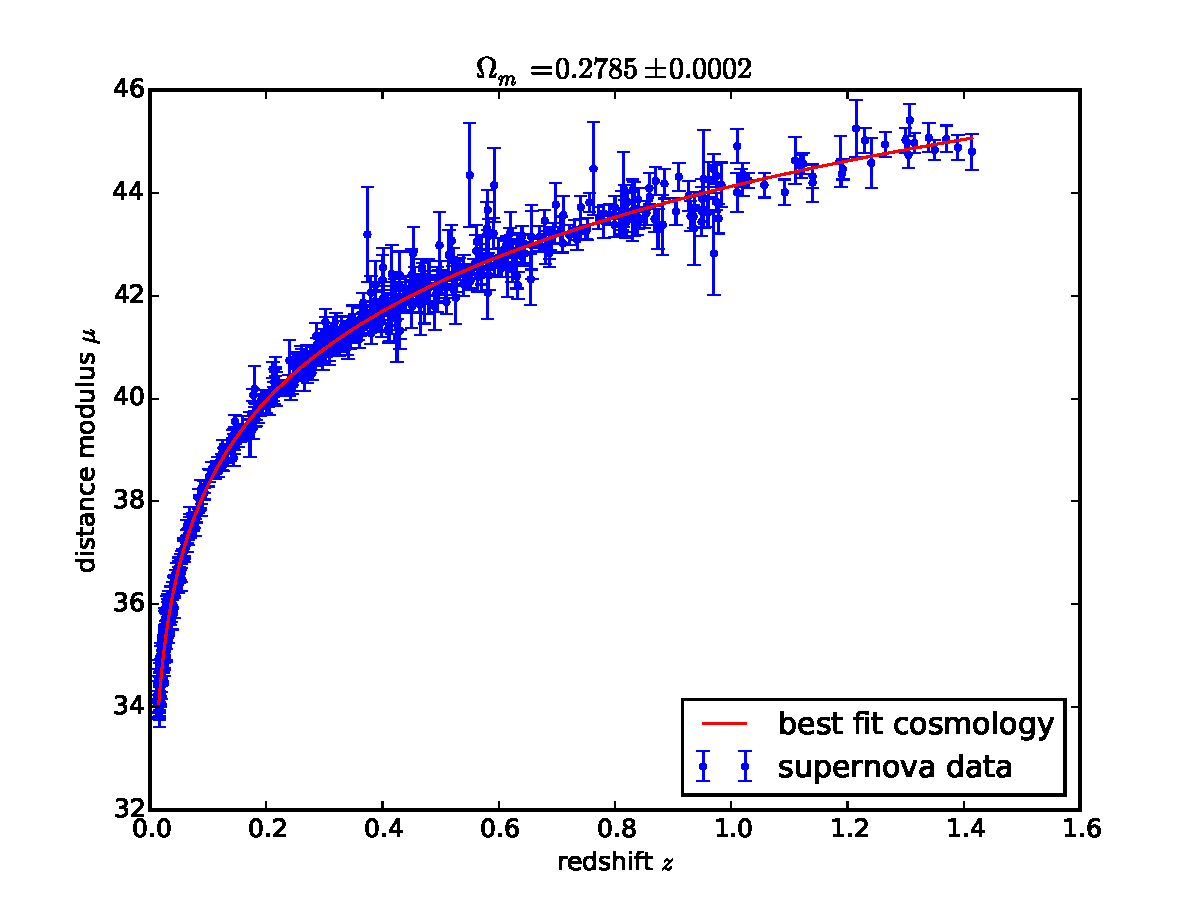
\includegraphics{./figures/supernova_fit.pdf}}
\caption{fit to the SCP-data in a FLRW-cosmology: $\Lambda$ is not zero}
\end{center}
\end{figure}

\item \question{precision of the measurement}\\
In running the script \path{supernova_likelihood.py} you can simultaneously fit $\Omega_m$ and $w$ to the data. It evaluates the likelihood $\mathcal{L}(\Omega_m,w)\propto \exp(-\chi^2(\Omega_m,w)/2)$, with 
\begin{equation}
\chi^2(\Omega_m,w) = \sum_{i=1}^{n_\mathrm{data}}\left(\frac{\mu_i-\mu(z_i,\Omega_m,w)}{\sigma_i}\right)^2
\end{equation}
for the $n_\mathrm{data}$ data points $\mu_i$ at the redshifts $z_i$. The probability that a parameter choice is true is reflected by the density of points.
\begin{enumerate}[(a)]
\item{What are the statistical errors on $\Omega_m$ and on $w$?}
\item{Why do you require more negative $w$ if $\Omega_m$ is larger?}
\end{enumerate}

\begin{figure}[h]
\begin{center}
\resizebox{9cm}{!}{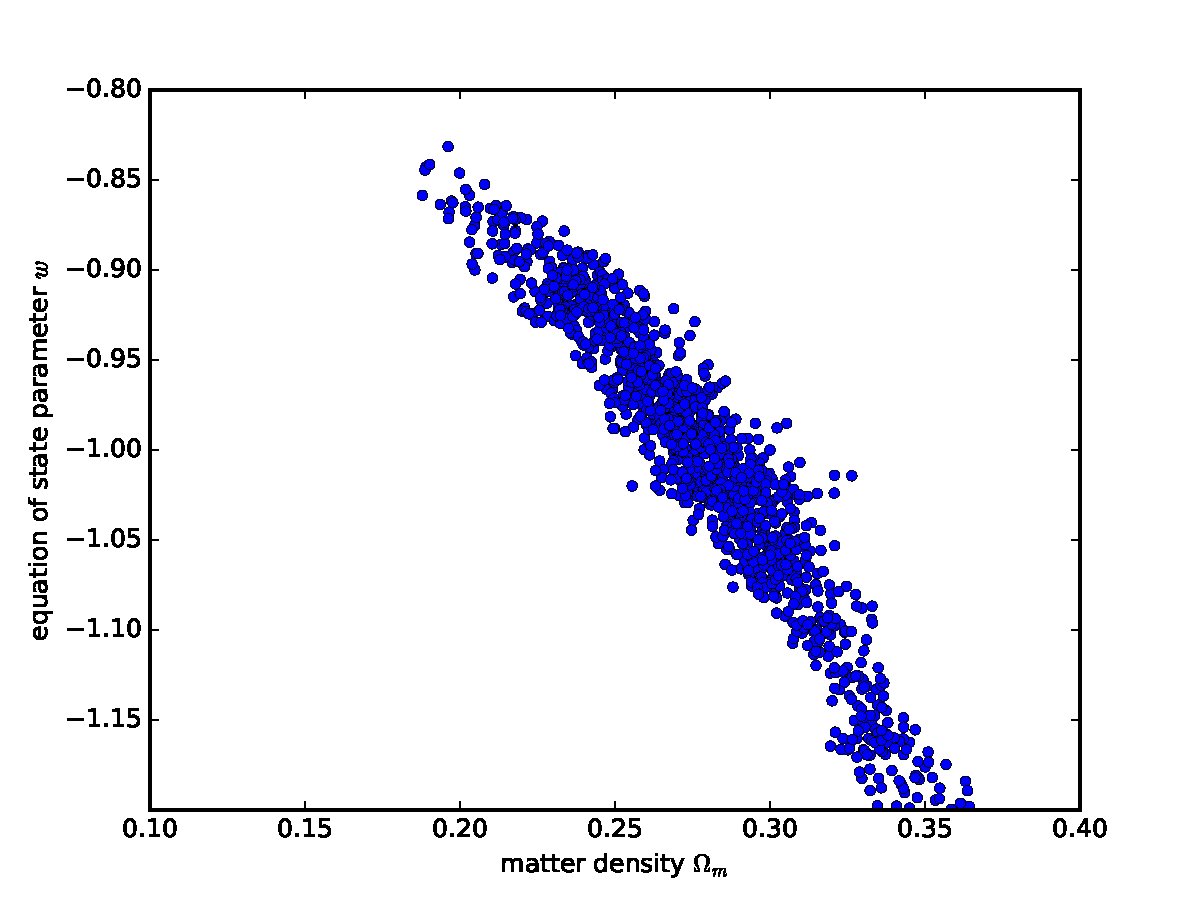
\includegraphics{./figures/supernova_mcmc.pdf}}
\caption{simultaneous measurement of $\Omega_\Lambda$ and $w$}
\end{center}
\end{figure}

\end{enumerate}
\end{document}
